\chapter{Baza danych}



Bazy danych pełnią kluczową rolę w strukturze wielu aplikacji, umożliwiając składowanie, organizację i efektywne zarządzanie danymi. Dzięki nim możliwe jest elastyczne dodawanie nowych informacji oraz rozwijanie funkcjonalności systemu. Struktury baz danych są zoptymalizowane pod kątem efektywnego przeszukiwania i pobierania danych, co przyczynia się do wydajnego działania aplikacji. Dodatkowo, istnieje szereg narzędzi, takich jak Spring Boot i Hibernate (tabela \ref{tab:zestawienie_narzędzi})
,które ułatwiają integrację z bazami danych, usprawniając tym samym proces ich obsługi.

\section{Model bazy danych}

\subsection{Opisy encji urządzeń}
W celu zdefiniowania struktury bazy danych, został stworzony diagram związków encji (ER), przedstawiony na rysunku \ref{ErDiagram_etykieta}. Diagram ten ilustruje, jakie typy danych są przechowywane w poszczególnych tabelach, a także jakie relacje zachodzą między tymi tabelami. Warto zaznaczyć, że ze względu na brak domyślnego wsparcia dla dziedziczenia tabel w relacyjnych bazach danych, zdecydowano się skorzystać z mechanizmu dziedziczenia dostępnego w Hibernate. W dalszej części rozdziału został omówiony schemat dziedziczenia.

W systemie istnieją różne rodzaje urządzeń, z których każdy jest reprezentowany przez odpowiadającą mu tabelę w bazie danych. Trzy główne kategorie urządzeń to: \textbf{computer (komputer), tablet (tablet)} oraz \textbf{other\_device (inne urządzenie)}. Wszystkie te kategorie dziedziczą swoje cechy od wspólnej tabeli o nazwie \textbf{device\_core}, która stanowi rdzeń dla wszystkich urządzeń.

Wspólny rdzeń, reprezentowany przez tabelę device\_core, zawiera parametry, które są dziedziczone przez wszystkie rodzaje urządzeń. Dzięki tej strukturze, każda tabela reprezentująca konkretny typ urządzenia posiada te same podstawowe atrybuty, ułatwiając jednolite zarządzanie nimi w systemie. Parametry wspólne dla wszystkich typów urządzeń obejmują: 
\begin{itemize}
	\item \texttt{ID} - identyfikator urządzenia
	\item \texttt{device\_type} - Typ urządzenia ułatwiający zarządzanie nimi w aplikacji klienckiej
	\item \texttt{device\_name} - Nazwa urządzenia
	\item \texttt{price} - Cena urządzenia
	\item \texttt{age} - Wiek urządzenia
	\item \texttt{office\_id} - identyfikator biura w którym znajduje się urządzenie
	\item \texttt{ready\_to\_lottery} - Informacja czy sprzęt jest gotowy do przeprowadzenia loterii
	\item \texttt{lottery\_date} - Data loterii w której odbyło się losowanie, jeżeli się nie odbyło to wartość jest pusta
	\item \texttt{is\_ordered} - Informacja czy sprzęt został już odebrany przez pracownika
\end{itemize}

Pozostałe tabele reprezentujące urządzenia rozszerzają informacje dostarczane przez rdzeń. Komputer dodatkowo posiada informacje odnośnie
\begin{itemize} % TO DO: poprawić czcionkę na maszynową jak w wyliczeniu powyżej (przypominam - czcionką maszynową piszemy kod, nazwy klas itd.)
	\item serial\_number - numer seryjny komputera
	\item model - model komputera
	\item operatinng\_system - system operacyjny zainstalowany na komputerze
	\item battery\_life - żywotność baterii
	\item cpu\_id - identyfikator reprezentujący procesor posiadany przez komputer
	\item storage\_id - identyfikator reprezentujący dysk posiadany przez komputer
	\item ram\_id - identyfikator reprezentujący pamięć RAM posiadaną przez komputer
\end{itemize}

Tablet posiada dodatkowo informacje odnośnie:
\begin{itemize}
	\item screen\_size- parametry wyświetlacza
	\item operatinng\_system - system operacyjny zainstalowany na tablecie
	\item battery\_life - żywotność baterii
\end{itemize}

Inne urządzenie natomiast posiada tylko pole additional\_info które pozwala na podanie szczególnych informacji urządzenia.

\subsection{Dziedziczenie tabel}
\label{dzedziczenie_hibernate:label}
Projektowany system powstał z myślą możliwości łatwego rozszerzania. Wykorzystanie tabeli \textbf{device\_core} ułatwi dodanie ewentualnych tabel potomnych. Kod tabeli nadrzędnej device\_core umożliwi wykonanie ogólnych operacji, co zapobiegnie powielaniu kodu oraz umożliwi dodanie tabel spełniających już funkcjonalności tabeli device\_core. Ważnym aspektem projektu jest zapewnienie unikalności kluczy w kontekście schematu dziedziczenia, szczególnie w przypadku użycia Hibernate z modelem \textbf{table~per~class}. W tym podejściu każda klasa dziedzicząca, tak jak computer, tablet, czy other\_device, ma swój własny identyfikator, ale także dziedziczy z klasy nadrzędnej. Hibernate automatycznie zarządza unikalnością kluczy dla całej hierarchii dziedziczenia, eliminując ryzyko konfliktów kluczy pomiędzy różnymi klasami. W praktyce, w bazie danych dla każdej klasy dziedziczącej, a także dla samej klasy device\_core, zostaną utworzone oddzielne tabele. Tabele te zawierają wszystkie pola związane z daną klasą, a Hibernate zarządza relacjami między nimi. W przypadku klasy device\_core, tabela zawiera podstawowe atrybuty wspólne dla wszystkich typów urządzeń, takie jak device\_name, price, age, itp. Przykład implementacji takiego dziedziczenia znajduje się w listingach kodu \ref{entity_deviceCore} i \ref{entity_computer}
\newline
Dla klas dziedziczących, takich jak \textbf{computer, tablet czy other\_device}, Hibernate generuje tabele z dodatkowymi kolumnami specyficznymi dla danej klasy, takimi jak serial\_number czy screen\_size. W efekcie każda tabela reprezentuje pełne zestawienie danych związanych z danym rodzajem urządzenia.


\begin{figure}[h]
    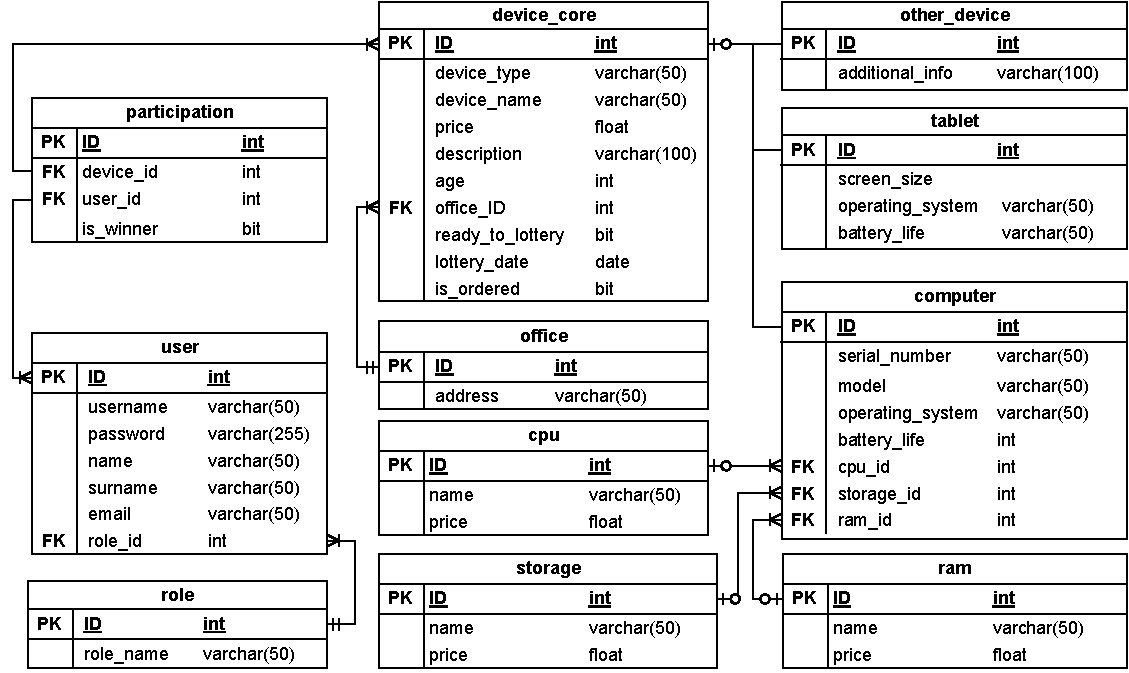
\includegraphics[width=\linewidth]{rys04/ER_Diagram.pdf}
    \caption{Diagram związków encji}
    \label{ErDiagram_etykieta}
\end{figure}

\section{Tworzenie bazy danych}
W tworzeniu baz danych istnieją dwa podejścia: code first i database first. W implementacji systemu wykorzystane zostało podejście database first. Daje do w początkowym etapie projektowania większą przejrzystość danych. Po stworzeniu modelu można potem skorzystać z gotowych narzędzi które pozwolą automatycznie wygenerować kod odzwierciedlający model danych.

Przy tworzeniu bazy danych wykorzystywanym narzędziem jest SSMS \ref{ssms:label}. 
Na początek stworzono tabele na podstawie diagramu związków encji \ref{ErDiagram_etykieta} oraz określono jej relacje. Przykład tworzenia encji oraz jej relacji znajduje się na poniższych rysunkach.

\begin{figure}[htb]
  \centering
	\begin{tabular}{@{}ll@{}}
	a) & b) \\
  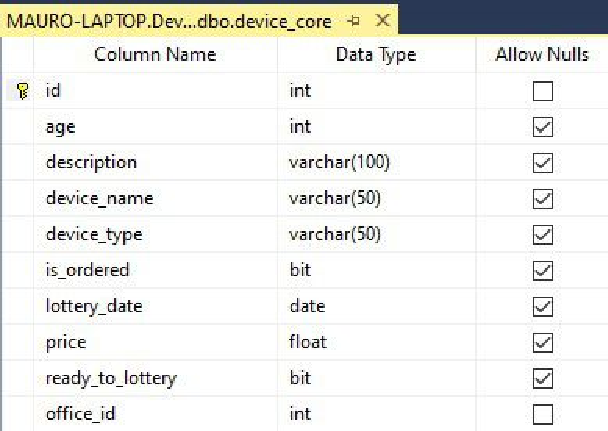
\includegraphics[width=0.475\textwidth]{rys04/design.pdf} & 
	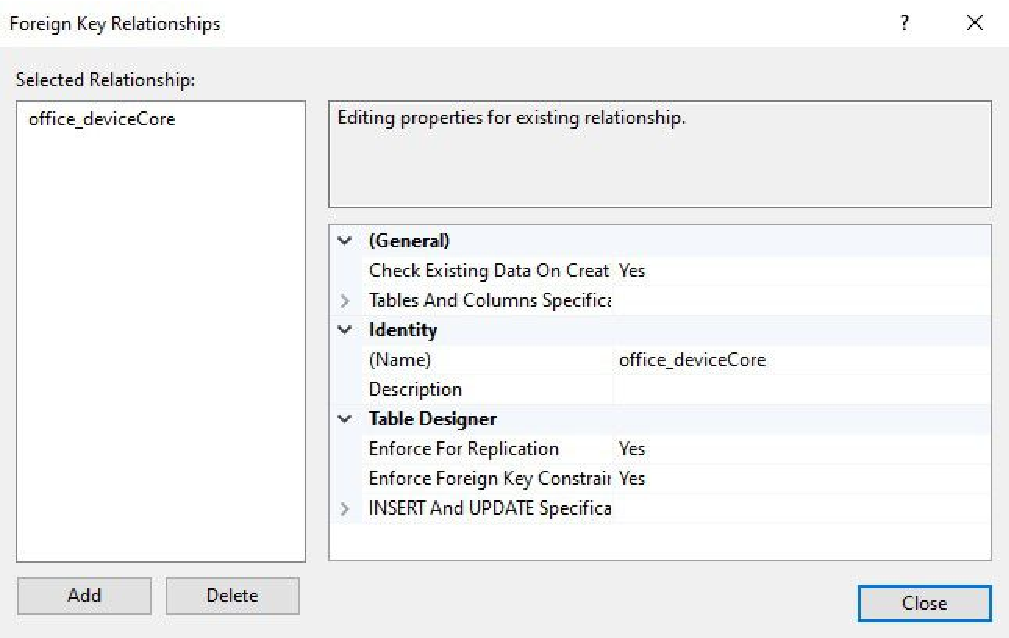
\includegraphics[width=0.475\textwidth]{rys04/relation.pdf}
	\end{tabular}
  \caption{Tworzenie bazy danych SSMS a) model, b) definiowanie relacji}
  \label{ssms_tworzenie:label}
\end{figure}

Po stworzeniu wszystkich tabel możliwe jest wygenerowanie kodu. Wykorzystano do tego plugin JPA Buddy oraz wbudowane narzędzia Intelij. Upraszcza to proces implementacji systemu. Ponizej przedstawiono sposób generowania kodu encji dla klasy computer.

\begin{figure}[h]
		\centering
    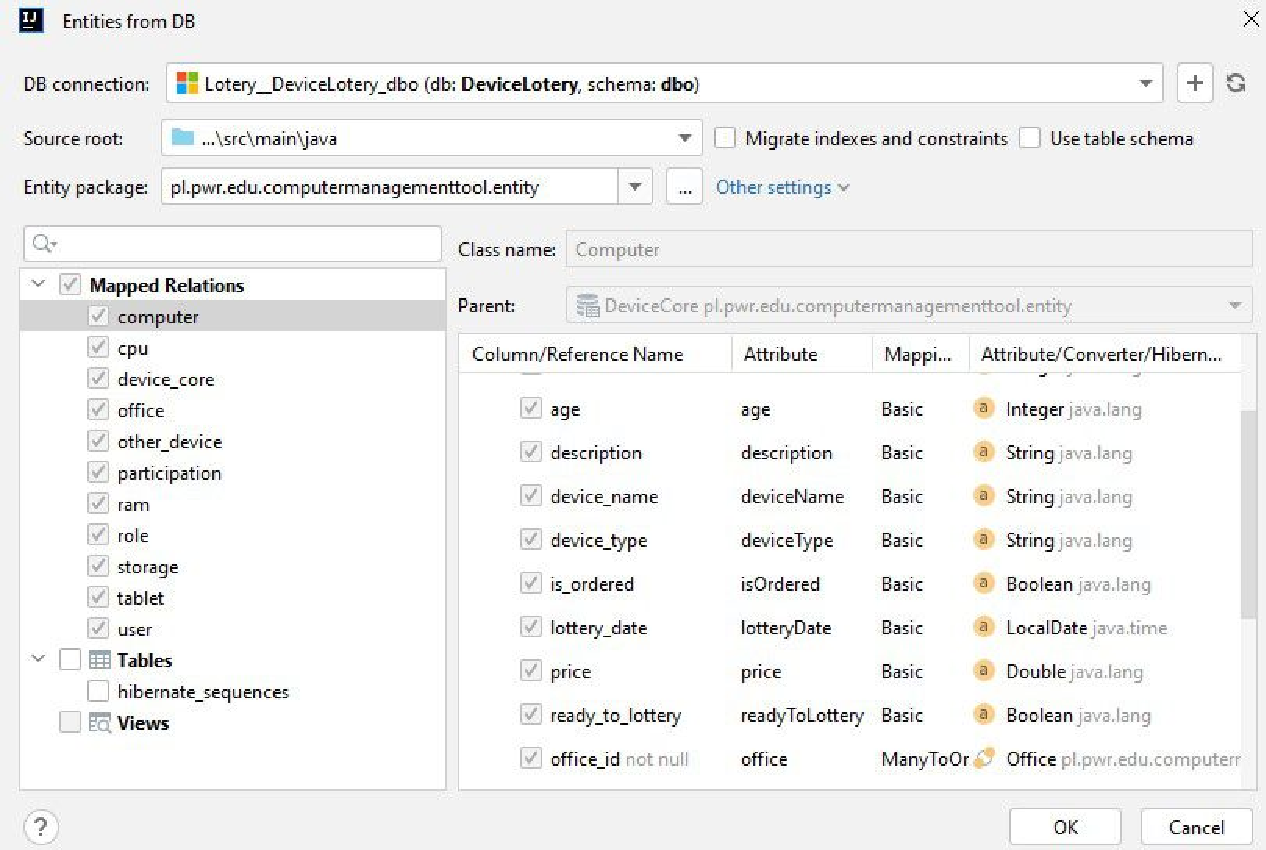
\includegraphics[width=0.7\linewidth]{rys04/generate.pdf}
    \caption{Generowaniu kodu na podstawie tabeli computer przy użyciu Intelij Idea}
    \label{generate:label}
\end{figure}

Tworzenie w ten sposób początkowej struktury projektu jest bardzo pomocne. Jednak kiedy definiuje się sposób dziedziczenia tabel to jedynym sposobem jest zdefiniowanie relacji wykorzystując Hibernate. O sposobie dziedziczenia tabel przez Hibernate napisano na początku tego rozdziału \ref{dzedziczenie_hibernate:label} Szczegóły implementacji dotyczące klasy device\_core opisano w podrozdziale \ref{entity_deviceCore}. Odpowiednia konfiguracja projektu umożliwia aktualizowanie struktury bazy danych. Możliwe dzięki temu jest wyeliminowanie nadmiarowego kodu oraz skorzystanie abstrakcji dostarczanej przez dziedziczenie. Gdy Hibernate zaktualizuje strukture bazy danych w SSMS automatycznie powstają odpowiednie tabele i relacje klas sprzętu. Zarządzanie unikalnością kluczy dla tych klas też jest możliwa tylko z poziomu kodu.
 
